\chapter{Introduction}

\section{Objet du projet}

Le but du projet est la réalisation de l’étude préalable préliminaire de la conception et de
l’automatisation du système d’information du domaine gestion des contrats de maintenance, chez SPIE SUD EST.

L'objectif du projet s'étend donc sur plusieurs points~:
\begin{itemize}
    \item Spécifications de solutions informatiques (standard, spécifique)~;
    \item Mise en oeuvre d’outils et de méthode de conception~;
    \item Modélisation de la solution (élaboration de scénarii)~;
    \item Choix des moyens, évaluation, etc~;
    \item Elaboration du plan qualité.
\end{itemize}

\paragraph{Note Importante} Le but du projet étant la réalisation d'une étude préalable, nous nous
limiterons aux phases de spécifications et de conception du système d’information. En d'autres termes,
nous ne prendrons donc pas en charge les phases suivantes dans l’étude préalable, c’est à dire~:
l’étude détaillée ainsi que la réalisation.


\section{Contexte général du projet}

\subsection{SPIE}

SPIE est une multinationale d'origine francaise, et réalisant encore aujourd'hui 62\% de son
chiffre d'affaire en France, 25\% en Europe et 13\% hors Europe. Son objectif est d'améliorer le confort
de tous les jours via divers systèmes, en réalisant 66\% de son chiffre d'affaire par la maintenance de ceux-ci.

SPIE est composé des services~:

\begin{itemize}
    \item Direction Générale (DG)~;
    \item Direction des Ressources Humaines (DRH)~;
    \item Direction Administrative et Financière~;
    \item Direction de la Stratégie et du Développement~;
    \item Services Régionaux~:
    \begin{itemize}
        \item SPIE Ouest-Centre~;
        \item SPIE Sud-Ouest~;
        \item SPIE Ile-de-France Nord-Ouest~;
        \item SPIE Est~;
        \item SPIE Sud-Est~;
        \item SPIE Europe du nord~:
        \begin{itemize}
            \item SPIE UK~;
            \item SPIE Nederland~;
            \item SPIE Belgium.
        \end{itemize}
    \end{itemize}
    \item Services de Spécialités~:
    \begin{itemize}
        \item SPIE Communications~;
        \item SPIE Oil \& Gas Service~;
        \item SPIE Nucléaire.
    \end{itemize}
\end{itemize}

\subsection{SPIE Sud-Est}

Dans le cadre du projet, nous nous intéresserons seulement au service régional SPIE SUD EST. Ce dernier
est composé de 3 directions de spécialités qui dépendent eux aussi de la Direction Générale~:

\begin{itemize}
    \item Génie climatique~;
    \item Industries~;
    \item Systèmes d’information \& transport.
\end{itemize}


La direction des Systèmes d’information \& transport assure le déploiement et l’exploitation des systèmes de
gestion~: Gestion des affaires et des moyens; Gestion des RH et payes; Comptabilité; Trésorerie ... De nombreux
progiciels sont intégrés au SI de SPIE.

\subsection{Exemples de contrat de maintenance}

SPIE réalisant 66\% de son chiffre d'affaire en maintenance, nous décrivons ici le fonctionnement des contrats de
maintenance. Ceux-ci sont donc composés de deux parties distinctes~:

\begin{description}
    \item[Partie forfaitaire~:] Concerne la maintenance préventive ou curative régulière des équipements
    après installation. Exemple, la maintenance de l'éclairage publique d'une ville.

    \item[Partie bon de commande~:] Concerne la maintenance curative exceptionnelle suite à un accident, vendalisme et
    même les travaux induits comme l'amélioration des installations ou le traitement de l’obsolescence.
\end{description}


\pagebreak
\section{Positionnement dans le cycle général du développement des SI}

SPIE est malheureusement équipé d'une variété de progiciels pour chacune des tâches, d'où son intention
de changer le tout pour un ERP unique (SAP).

\begin{figure}[h]
    \centering
    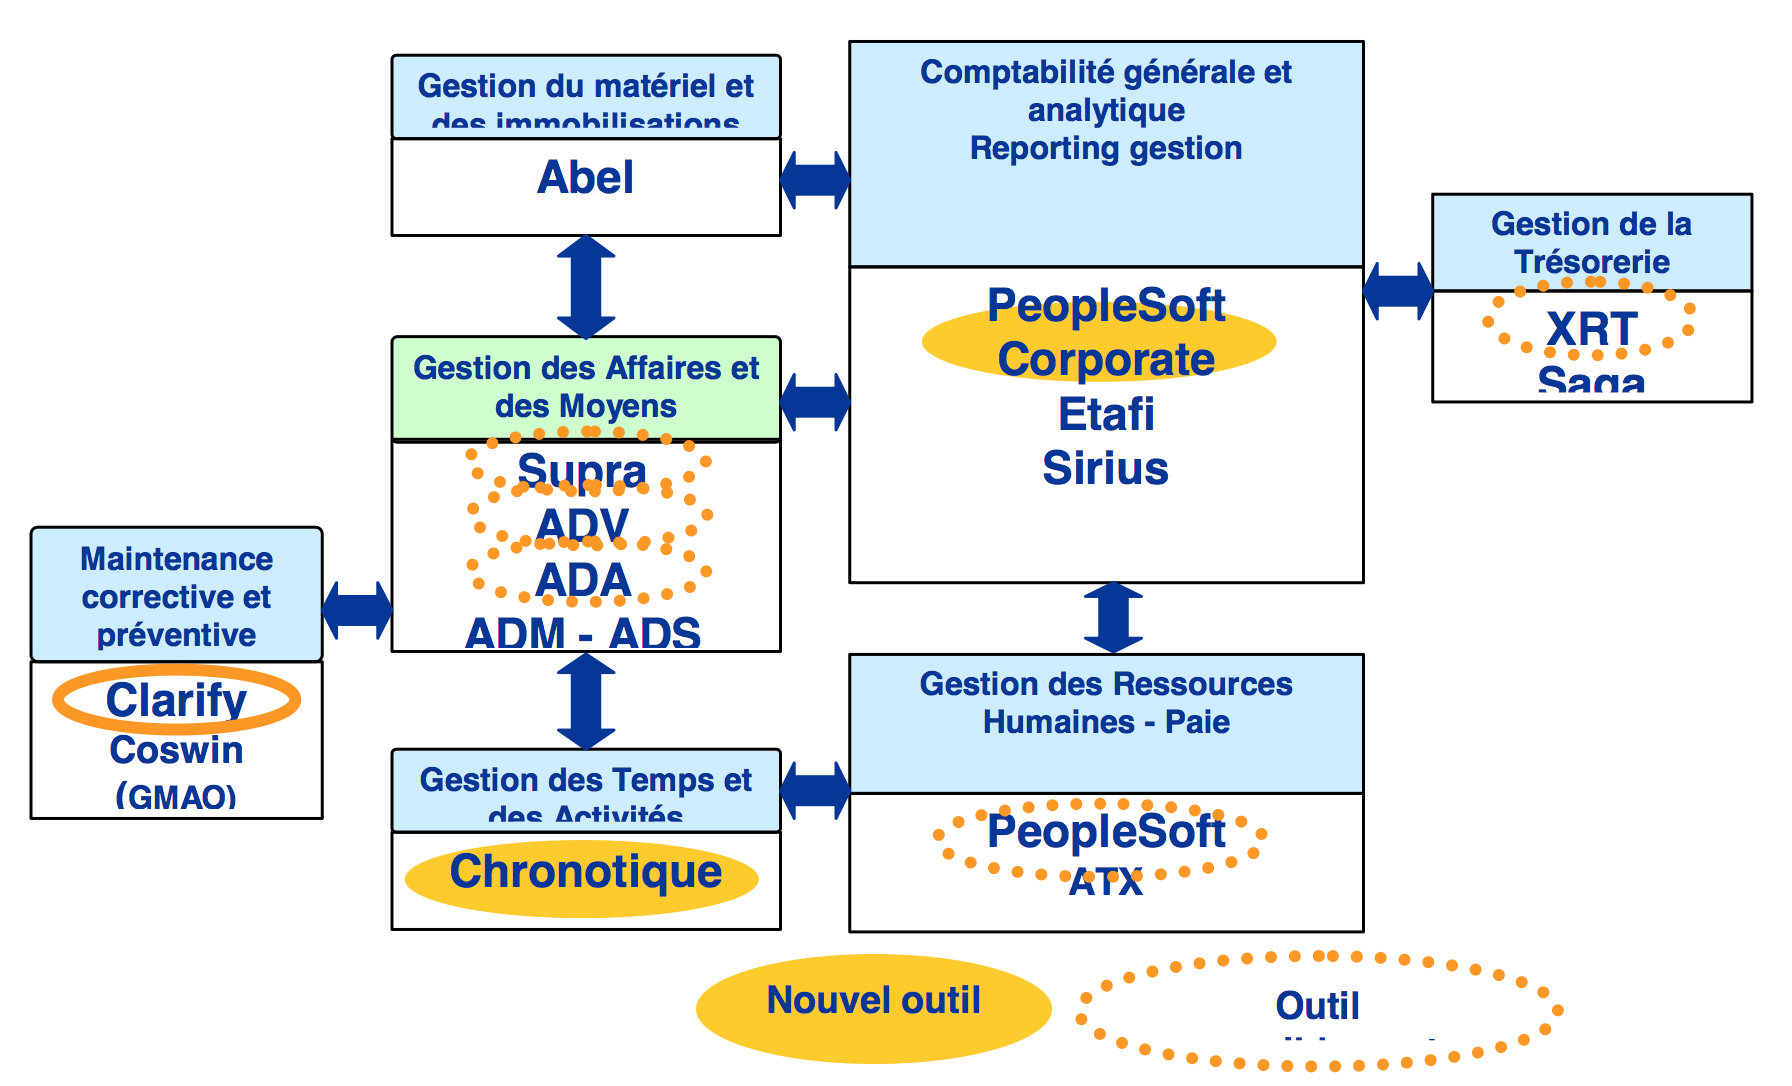
\includegraphics[width=140mm]{./images/A_SI_actuelles.png}
    \caption{Cartographie générale du SI de SPIE}
    \label{diagram:si_map}
\end{figure}

Les attentes du clients sont~:

\begin{itemize}
    \item Pour la solution standard : évoluer vers un ERP unique (SAP)
    \item Pour les opérations de maintenance : souhait de saisir les événements et les compte-rendus à la
    source (nomadisme)
\end{itemize}

